%!TEX root = ../summaries.tex

\chapter{Decomposing tasks for outer alignment}

\section{Factored cognition}

\url{https://ought.org/research/factored-cognition}


\subsection{Introduction}

\begin{itemize}
    \item \emph{One-step amplification}: agent has a number of copies of itself which work on sub-tasks with equal limitations on computational capacity.
    \item \emph{Iterated amplification}: this iterated.
    \item \emph{Factored cognition}: learning broken down like this into small and mostly independent tasks.
\end{itemize}


\subsection{Scalable mechanisms for solving cognitive tasks}

\begin{itemize}
    \item Want to find mechanisms for solving cognitive tasks which scale with respect to number of human work-hours and access to ML algorithms.
    \item Assumptions.
    \begin{enumerate}[label=(\arabic*)]
        \item\label{item:well-motivated; assumptions; factored cognition} Human workers well-motivated.
        \item\label{item:limited time; assumptions; factored cognition} Each only available for say 15 minutes.
        \item\label{item:same background; assumptions; factored cognition} Each has same background knowledge.
    \end{enumerate}
    \item Mechanism: \emph{Iterated Distillation-Amplification}.
    \item Example cognitive tasks.
    \begin{itemize}
        \item Read this book and tell me why $x$ did $y$.
        \item Provide a detailed analysis of the pros and cons of these two products.
        \item Tell me how to invest \$100k to achieve the most social good.
        \item Write a paper on NLP that substantially advances the state of the art.
    \end{itemize}
    \item Scalability.
    \begin{itemize}
        \item More resources $\rsa$ better results.
        \item Resources: human work-hours and ML algos.
        \item Better: more aligned with task-setter's interests.
        \item Scalability desirable because it helps turn thinking into a commodity.
        \item Scalable system automatically gets more helpful when we plug in more advanced ML systems.
    \end{itemize}
    \item Organizing human work on cognitive tasks.
    \begin{itemize}
        \item Scalability of single person doing task limited by number of hours available and ability to reason and learn.
        \item Scalability of group of people limited by communication and delegation.
        \item Doesn't discuss motivation problem (assumption \ref{item:well-motivated; assumptions; factored cognition}).
        \item How do we orchestrate people so that the output scales with number of people.
        \item Short-term context-free work.
        \begin{itemize}
            \item By assumption \ref{item:limited time; assumptions; factored cognition}, no worker has time to build up much context.
            \item Can we compose simple local tasks to solve a complex problem?
        \end{itemize}
        \item Coordination of short-term work as algorithm design.
        \begin{itemize}
            \item Take humans to be a function which takes a task string and outputs result (assumption \ref{item:same background; assumptions; factored cognition}).
            \item Can we mechanically compose calls to this stateless function to solve task?
            \item This is about algorithm design.
        \end{itemize}
        \item Matching the quality of any other approach to solving cognitive tasks.
        \begin{itemize}
            \item Want approach that scales with number of calls to function.
            \item Could compare to other ways of solving task.
            \begin{itemize}
                \item Is there a number of calls to function with means we can do as well as any other fixed solution?
                \item Problem: evaluating how well a task is solved a hard cognitive question.
                \item Problem: empirical content of solutions, which may include built-in solutions to some tasks.
            \end{itemize}
            \item Alternative: compare to subjective of idealised deliberation.
            \begin{itemize}
                \item Problem: this is exactly what we're trying to solve.
            \end{itemize}
            \item Best compromise: can we solve any task to arbitrary high quality?
            \begin{itemize}
                \item Unlikely to be the case: any task which involves learning could be done without learning.
                \item Might still be useful to aim for it, to get systems which scale well in practice, but have theoretical bounds.
                \item Also: might produce alternatives to solutions which are expensive to implement directly.
            \end{itemize}
        \end{itemize}
    \end{itemize}
    \item Applying machine learning to cognitive tasks.
    \begin{itemize}
        \item Scalability now also wrt to ML sophistication.
        \begin{itemize}
            \item Better priors.
            \item Better inference.
            \item Better training paradigms.
        \end{itemize}
        \item Approaches that don't scale.
        \begin{itemize}
            \item Training systems on $(\text{task}, \text{solution})$ pairs.
            \begin{itemize}
                \item Doesn't scale because we can't generate an arbitrary quantity of training data: can't generate solutions of arbitrarily high quality.
            \end{itemize}
            \item Reinforcement learning based on how good a solutions seems.
            \begin{itemize}
                \item Optimises for proxy to solution's goodness.
            \end{itemize}
        \end{itemize}
        \item An approach that might scale.
        \begin{itemize}
            \item Worthwhile to consider how to scalably apply current ML algos, assuming they only scale along the dimensions mentioned above.
            \item Iterated Distillation-Amplification.
            \begin{enumerate}[label=\arabic*.]
                \item Initialise fast ML $A$ randomly.
                \item Repeat:
                \begin{enumerate}[label=\alph*.]
                    \item Amplification: Build slow system which involves human making single step, with multiple calls to $A$.
                    \item Distillation: Retrain $A$ to imitate behaviour of this slow system.
                \end{enumerate}
            \end{enumerate}
            \begin{itemize}
                \item Depends on ability to decompose task into small context-free steps.
            \end{itemize}
        \end{itemize}
    \end{itemize}
\end{itemize}


\section{Recursively Summarizing Books with Human Feedback}

\url{https://arxiv.org/abs/2109.10862}


\subsection{Introduction}

\begin{itemize}
    \item Task: summarise whole book.
    \item Difficult to generate training data for whole task or evaluate model performance: human has to read entire book.
    \item Recursively splits task into smaller: summarise small section, summarise summaries etc.
    \item Humans can evaluate performance on smaller tasks.
    \item \emph{Scalable oversight}: scalably evaluating model performance.
    \item Single model for summarising.
    \item Trained using cross-entropy behavioural cloning (BC), and with reinforcement learning (RL).
    \item Obtain believable summaries for books containing 100,000s words.
    \item Qualitatively, summaries contain important details, but fail to put work in broader context.
    \item Qualitatively, model significantly outperforms baseline.
    \item RL has better scaling properties.
    \item Evaluate summaries on NarrativeQA dataset: zero-shot model taking summaries as input achieves good results on question-answers.
\end{itemize}


\subsection{Approach}

\begin{itemize}
    \item General approach: single model does both the decomposition and responding to subtasks.
    \item This model: breaks text into chunks based on max chunk length.
    \item Problem: summarisers in middle of book lack sufficient context to accurately summarise their chunks.
    \begin{itemize}
        \item Solution: add previous context: summaries of preceding parts of the same depth.
    \end{itemize}
    \item Uniformity: all nodes in the decomposition tree are very similar.
    \item Training.
    \begin{itemize}
        \item Start with pretrained language model GPT-3 and pool of human labellers.
        \item Collect demonstrations and train using behavioural cloning.
        \item Then repeat iterations of reward learning and reinforcement learning.
        \item To learn the reward, collect comparisons from humans.
        \item RL optimises the reward plus KL term for initial policy.
        \item Auto-induced distributional shift.
        \begin{itemize}
            \item Outputs of model itself are outside the training distribution.
            \item Likely more severe later on in the book and higher up the tree.
            \item Did not measure severity.
            \item Found that more training on level 0 yielded better results on level 1.
        \end{itemize}
        \item Training curriculum.
        \begin{itemize}
            \item \emph{First subtree}: first height-1 node and its height-0 children.
            \item \emph{First leaves}: height-0 children in first subtree.
            \item First trained exclusively on first leaves.
            \item Then moved to first subtree.
            \item At this point, model can already generalise to full tree.Training dataset
            \item Curriculum changes made in ad-hoc manner.
        \end{itemize}
    \end{itemize}
    \item Advantages of decomposition.
    \begin{itemize}
        \item Easier to collect human feedback.
        \item Empowers human to do or evaluate part of task themself.
        \item Easier to trace model thinking and debug.
        \item Generalises quickly to longer books.
    \end{itemize}
\end{itemize}


\subsection{Task details}

\begin{itemize}
    \item Training dataset.
    \begin{itemize}
        \item Primarily fiction, over 100K words on average.
        \item Only use narrative works.
        \begin{itemize}
            \item Harder to summarise.
        \end{itemize}
    \end{itemize}
    \item Summarization task.
    \begin{itemize}
        \item Aim to summarise abstractly, rather than listing events.
        \item Primary metric: overall summary quality on a 1-7 Likert scale, on books neither in GPT-3 training set nor model training set.
        \item Aim to compress text by factor of 5--10$\times$.
        \item Labellers asked to judge conditioned on length: \textquote{how good is this summary, given that it is X words long?}
        \item Labellers only consider quality wrt to input, not wrt to subset of book in its context.
    \end{itemize}
\end{itemize}


\subsection{Results}

\begin{itemize}
    \item Methodology
    \begin{itemize}
        \item Used 40 most popular books published in 2020.
        \item Two labellers read each book, then rate model-produced summaries and that of other labeller.
        \item Labeller agreement on relative quality of model-produced summaries nearly 80\%.
        \item Evaluate 175B and 6B parametered models.
        \item For each, evaluate three training modes:
        \begin{itemize}
            \item RL on whole tree.
            \item RL on first subtree.
            \item BC on whole tree.
        \end{itemize}
        \item Findings.
    \end{itemize}
    \begin{itemize}
        \item See \cref{fig:likert} for distributions of likert scores for various summarisers.
        \item Likert scores for whole book significantly worst than for individual task. Errors accumulate.
    \end{itemize}
\end{itemize}

\begin{figure}
    \centering
    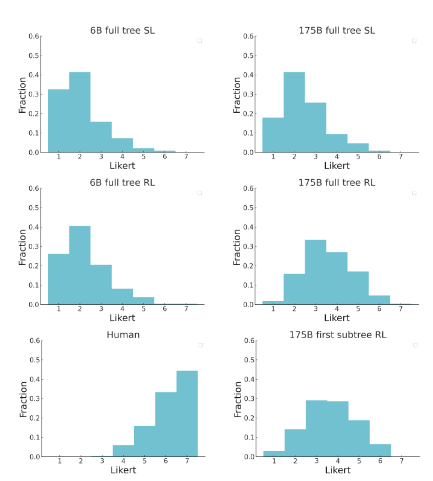
\includegraphics[width=.95\linewidth]{images/likert-distros.png}
    \caption{Likert distributions for various summarisers, taken from the paper}
    \label{fig:likert}
\end{figure}


\section{Supervising strong learners by amplifying weak experts}

\url{https://arxiv.org/abs/1810.08575}

\begin{itemize}
    \item Proposes \emph{Iterated Amplification}: progressively builds up training signal for complex tasks by combining solutions to simpler ones.
\end{itemize}

\subsection{Introduction}

\begin{itemize}
    \item Concerned with tasks where specifying reward function is beyond human capability (for single human, and quickly enough).
    \begin{itemize}
        \item Economic policy decisions.
        \item Doing science.
        \item Security of large network of computers.
    \end{itemize}
    \item Will allow expanding applicability of AI.
    \item Will allow building robustly safe systems.
    \begin{itemize}
        \item In practice, find short-term proxy for what we want.
        \item Aggressively optimising this can lead to pathological behaviour.
    \end{itemize}
    \item Iterated Amplification.
    \begin{itemize}
        \item Human agent $H$ trains ML agent $X$.
        \item $H$ demonstrates target behaviour using several copies of $X$.
        \item Write $\Amplify^H(X)$ for this composite system.
        \item $X$ learns from $\Amplify^H(X)$ in normal way.
        \item Need to make three design decisions.
        \begin{itemize}
            \item What tasks to solve?
            \item To do we construct $\Amplify^H(X)$?
            \item How does $X$ learn from $\Amplify^H(X)$?
        \end{itemize}
        \item Training process.
        \begin{itemize}
            \item $X$ initially behaves randomly, so $\Amplify^H(X)$ is the same as $H$.
            \item As $X$ becomes more powerful, role of $H$ transitions to coordinating a groups of $X$'s.
            \item Eventually the task of `find suitable subtasks' may be delegated to $X$.
            \item As long as $\Amplify^H(X)$ is more powerful than $X$, it provides a useful training signal.
        \end{itemize}
        \item No external reward function: this is implicit in $H$'s behaviour.
        \begin{itemize}
            \item Aim: $X$ learns goal at the same time as learning to act competently.
        \end{itemize}
    \end{itemize}
\end{itemize}


\section{AI Safety via Debate}

\url{https://openai.com/blog/debate/}

\begin{itemize}
    \item Proposes method of aligning agents using debate games.
    \item Idea: two agents debate correct output in natural language, and human judges who wins.
    \item Motivation: while human cannot effectively explore/understand whole solution space, the debate of two `expert' agents provides a heuristic for solution quality.
    \item Debate can focus on simpler factual claims, eventually producing sequence which human can effectively judge.
    \item Proof of concept using sparse MNIST classifier.
    \begin{itemize}
        \item Judge AI trained to classify digits from small subset of pixels.
        \item Two agents Alice and Bob.
        \item Alice tries to deceive judge, Bob tries to honestly persuade.
        \item Take turns revealing true white pixel.
        \item Judge judges bases on final set of six pixels.
        \item Debate turns 59.4\% accurate judge into 88.9\% accurate. 
    \end{itemize}
    \item Limitations and future work.
    \begin{itemize}
        \item Real test: powerful AIs debating using natural language with human interpreter.
        \item Important to test debates where human biases play a role.
        \item Debate cannot address distributional shift or adversarial examples.
        \item No guarantee debate will arrive at optimal play.
        \item Debate-trained agents use more computation.
        \item Humans may be poor judges.
    \end{itemize}
\end{itemize}